\documentclass[10pt,a4paper]{amsart}
\usepackage[margin=19mm]{geometry}
\usepackage{amsmath,amssymb,mathtools}
\usepackage[scr=rsfs,cal=euler]{mathalfa}
\usepackage{xfrac}
\usepackage[unicode,hidelinks,bookmarks=false]{hyperref}
\newcommand{\ie}{i.e.\ }
\newcommand{\cf}{cf.\ }
\newcommand{\resp}{respectively\ }
\newcommand{\Subsection}{\subsection}
\providecommand{\nobreakdash}{\nobreak\hbox{-}}
\setlength{\emergencystretch}{2em}
\multlinegap0pt
\usepackage{tikz}
\usepackage{float}
\usepackage{amssymb}
\usepackage[normalem]{ulem}
\usepackage[all]{xy}
\newtheorem{lemma}{Lemma}
\newtheorem{scope}{Scope}
\title{Independence of homogeneous GKM manifolds and symmetric spaces}
\author{Shintaro Kuroki, Grigory Solomadin}
\date{Source: arXiv:2602.07734v1 (CC BY 4.0)}
\begin{document}
\maketitle

\noindent\emph{Source and licence.} Independence of homogeneous GKM manifolds and symmetric spaces. Version arXiv:2602.07734v1 (CC BY 4.0), distributed by arXiv under the Creative Commons Attribution 4.0 International licence, http://creativecommons.org/licenses/by/4.0/, as recorded in the arXiv licence metadata for this exact version and shown on the abstract page https://arxiv.org/abs/2602.07734v1. Full licence notice: \texttt{licenses/arxiv-2602.07734-CC-BY-4.0.txt}.\par\smallskip

\noindent\textit{Editorial scope.} Counted unit: the article's lemma lm:23dep (source0.tex lines 1052--1168). The article's complete original proof of it is delivered with it (source0.tex lines 1169--1338, one \texttt{proof} environment of 170 lines). No mathematics is written, repaired or re-derived: the statement and the proof are the article's own lines, in the article's own notation, and no retained line is substituted or re-flowed.  No further source-local context is needed: every cross-reference of every retained line resolves inside the two delivered spans.  Nothing was omitted from any retained span, so the package carries no omission record.  No retained line contains a citation, so the wrapper carries no bibliography and no bibliography entry.  The retained lines contain the article's own diagram code, which the wrapper typesets with the standard tikz packages; no image file is delivered and the package declares no asset dependency.  Editorial formatting only, in addition: an AMS \texttt{amsart} preamble that restates the article's own declarations and macros used by the retained lines, namely the environments \texttt{lemma}, \texttt{scope} on separate counters, together with the standard packages those lines need.  The retained environments print in this document as Lemma 1, Scope 1 in order of appearance, whereas the article prints the same items with the numbering of its own full document.  The complete native source of the article as distributed in the arXiv e-print for this exact version is bundled unchanged as \texttt{sources/194207/source0.tex}.
\begin{lemma}\label{lm:23dep}
Let $G$ be a simple Lie group of type $A$--$D$, and $H$ be
its proper maximal connected (closed) maximal rank subgroup.
Then one has the following:
\begin{enumerate}
\item $k(G/H)=2$ if and only if the weighted signed graph $\Gamma(G,H)$ has a subgraph (with weighted vertices) appeared in Figure~\ref{example_weighted_vertex}, where $i<j<k$.
%%%%%%%%%%%%%%%%%%%%%%%%%%%%%%%%%%%%%%%%%%%%%%%%%%%%%%%%%%%%%%%%%%%%%%%%%%%
% Figure 3
%%%%%%%%%%%%%%%%%%%%%%%%%%%%%%%%%%%%%%%%%%%%%%%%%%%%%%%%%%%%%%%%%%%%%%%%%%%
\begin{figure}[H]
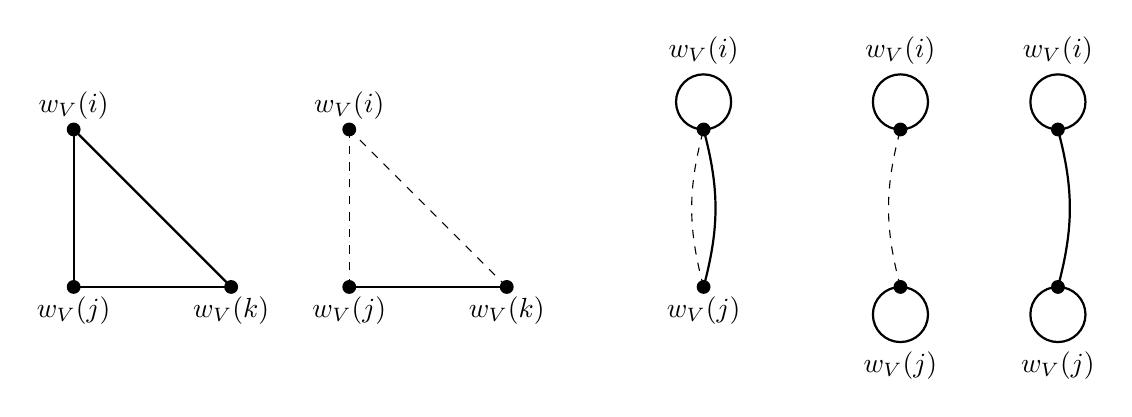
\begin{tikzpicture}
\begin{scope}[xscale=0.5, yscale=0.5]

\fill(-2,-2)circle (5pt);
\fill(-2,2)circle (5pt);
\fill(2,-2)circle (5pt);
\draw[thick](-2,-2)--(-2,2);
\node[above] at (-2,2) {$w_{V}(i)$};
\draw[thick](2,-2)--(-2,2);
\node[below] at (-2,-2) {$w_{V}(j)$};
\draw[thick](-2,-2)--(2,-2);
\node[below] at (2,-2) {$w_{V}(k)$};

\fill(5,2)circle (5pt);
\fill(5,-2)circle (5pt);
\fill(9,-2)circle (5pt);
\draw[dashed](5,-2)--(5,2);
\node[above] at (5,2) {$w_{V}(i)$};
\draw[dashed](9,-2)--(5,2);
\node[below] at (5,-2) {$w_{V}(j)$};
\draw[thick](9,-2)--(5,-2);
\node[below] at (9,-2) {$w_{V}(k)$};

\fill(14,2)circle (5pt);
\fill(14,-2)circle (5pt);
\draw[thick](14,-2)to[out=75,in=-75](14,2);
\draw[dashed](14,-2)to[out=105,in=-105](14,2);
\draw[thick](14,2.7) circle [x radius=0.7cm, y radius=0.7cm];
\node[above] at (14,3.4) {$w_{V}(i)$}; 
\node[below] at (14,-2) {$w_{V}(j)$};

\fill(19,2)circle (5pt);
\fill(19,-2)circle (5pt);
\draw[dashed](19,-2)to[out=105,in=-105](19,2);
\draw[thick](19,2.7) circle [x radius=0.7cm, y radius=0.7cm];
\node[above] at (19,3.4) {$w_{V}(i)$};
\draw[thick](19,-2.7) circle [x radius=0.7cm, y radius=0.7cm];
\node[below] at (19,-3.4) {$w_{V}(j)$};

\fill(23,2)circle (5pt);
\fill(23,-2)circle (5pt);
\draw[thick](23,-2)to[out=75,in=-75](23,2);
\draw[thick](23,2.7) circle [x radius=0.7cm, y radius=0.7cm];
\node[above] at (23,3.4) {$w_{V}(i)$};
\draw[thick](23,-2.7) circle [x radius=0.7cm, y radius=0.7cm];
\node[below] at (23,-3.4) {$w_{V}(j)$};

\end{scope}
\end{tikzpicture}
\caption{$2$-independent subgraphs.} 
\label{example_weighted_vertex}
\end{figure}
\item $k(G/H)=3$ if the weighted signed graph $\Gamma(G,H)$ has neither of the subgraphs (with weighted vertices) depicted in Figure~\ref{example_weighted_vertex} but has a weighted subgraph appeared in  Figure~\ref{example_weighted_vertex2}, where $i<j<k<l$.
%%%%%%%%%%%%%%%%%%%%%%%%%%%%%%%%%%%%%%%%%%%%%%%%%%%%%%%%%%%%%%%%%%%%%%%%%%%
% Figure 4
%%%%%%%%%%%%%%%%%%%%%%%%%%%%%%%%%%%%%%%%%%%%%%%%%%%%%%%%%%%%%%%%%%%%%%%%%%%
\begin{figure}[H]
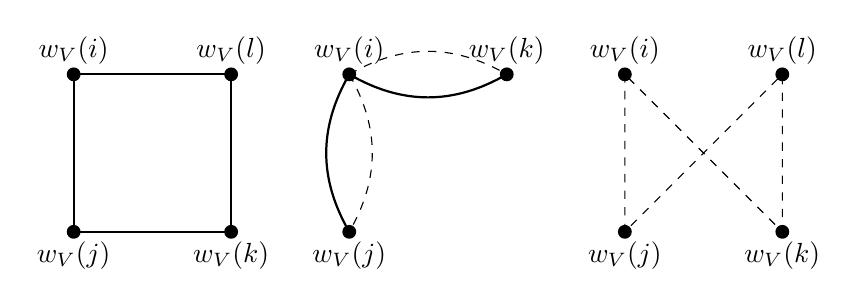
\begin{tikzpicture}
\begin{scope}[xscale=0.5, yscale=0.5]

\fill(-2,-2)circle (5pt);
\fill(-2,2)circle (5pt);
\fill(2,-2)circle (5pt);
\fill(2,2)circle (5pt);
\draw[thick](-2,-2)--(-2,2)--(2,2)--(2,-2)--cycle;
\node[above] at (-2,2) {$w_{V}(i)$};
\node[below] at (-2,-2) {$w_{V}(j)$};
\node[below] at (2,-2) {$w_{V}(k)$};
\node[above] at (2,2) {$w_{V}(l)$};

\coordinate (A) at (5,2);
\coordinate (B) at (5,-2);
\coordinate (C) at (9,2);
\fill(A)circle (5pt);
\fill(B)circle (5pt);
\fill(C)circle (5pt);
\draw[thick](A)to[out=240,in=120](B);
\node[above] at (A) {$w_{V}(i)$};
\draw[dashed](A)to[out=300,in=60](B);
\node[below] at (B) {$w_{V}(j)$};
\draw[thick](A)to[out=330,in=210](C);
\node[above] at (C) {$w_{V}(k)$};
\draw[dashed](A)to[out=30,in=150](C);

\coordinate (a) at (12,2);
\coordinate (b) at (12,-2);
\coordinate (c) at (16,-2);
\coordinate (d) at (16,2);
\fill(a)circle (5pt);
\fill(b)circle (5pt);
\fill(c)circle (5pt);
\fill(d)circle (5pt);

\draw[dashed] (a)--(b)--(d)--(c)--(a);

\node[above] at (a) {$w_{V}(i)$};
\node[below] at (b) {$w_{V}(j)$};
\node[below] at (c) {$w_{V}(k)$};
\node[above] at (d) {$w_{V}(l)$};

\end{scope}
\end{tikzpicture}
\caption{$3$-independent subgraphs.}
\label{example_weighted_vertex2}
\end{figure}
\end{enumerate}
\end{lemma}

\begin{proof}
For $\Gamma(G,H)$, since the statement $(2)$ is straightforward, we only prove the statement $(1)$.
If there is a subgraph which is drawn in Figure~\ref{example_weighted_vertex}, then by the definition of weighted signed graphs, $\Gamma(G,H)$ is $2$-independent, i.e., $k(G/H)=2$. 
 
Assume that $k(G/H)=2$, i.e., there are three edges (or loops) that are 2-independent in $\Gamma(G,H)$.
Let $\Gamma'$ be a subgraph in $\Gamma(G,H)$ consisting of such three eges (or loops). 
We first claim that $\Gamma'$ has two or three vertices.
It is easy to verify that a subgraph in $\Gamma(G,H)$ with three edges (or loops) and more than four vertices is one of the following graphs: 
\begin{itemize}
\item three parallel edges (six vertices);
\item two parallel edges and a separate loop (five vertices);
\item two connected edges with 3 vertices (i.e., V shape) and a separate edge (five vertices);
\item two connected edges with 3 vertices (i.e., V shape) and a separate loop (four vertices);
\item one edge and two separate loops (four vertices);
\item one multiple edge and a separate edge (four vertices);
\item three connected edges with 4 vertices (i.e., N shape)
\end{itemize}
By the definition of weighted signed graphs, all weights of these graphs correspond to linearly independent vectors. 
Hence, there are no subgraphs of three 2-independent edges (or loops) with more than 4 vertices.

If $\Gamma'$ consists of three vertices without loops, then by the definition of weighted signed graph there are the following four types in Figure~\ref{three_vertices} for some edges $i<j<k$.
%%%%%%%%%%%%%%%%%%%%%%%%%%%%%%%%%%%%%%%%%%%%%%%%%%%%%%%%%%%%%%%%%%%%%%%%%%%
% Figure 5
%%%%%%%%%%%%%%%%%%%%%%%%%%%%%%%%%%%%%%%%%%%%%%%%%%%%%%%%%%%%%%%%%%%%%%%%%%%
\begin{figure}[H]
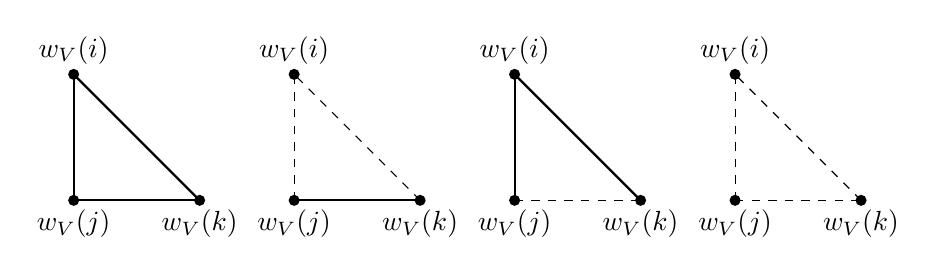
\begin{tikzpicture}
\begin{scope}[xscale=0.4, yscale=0.4]

\fill(-2,-2)circle (5pt);
\fill(-2,2)circle (5pt);
\fill(2,-2)circle (5pt);
\draw[thick](-2,-2)--(-2,2);
\node[above] at (-2,2) {$w_{V}(i)$};
\draw[thick](2,-2)--(-2,2);
\node[below] at (-2,-2) {$w_{V}(j)$};
\draw[thick](-2,-2)--(2,-2);
\node[below] at (2,-2) {$w_{V}(k)$};

\fill(5,2)circle (5pt);
\fill(5,-2)circle (5pt);
\fill(9,-2)circle (5pt);
\draw[dashed](5,-2)--(5,2);
\node[above] at (5,2) {$w_{V}(i)$};
\draw[dashed](9,-2)--(5,2);
\node[below] at (5,-2) {$w_{V}(j)$};
\draw[thick](9,-2)--(5,-2);
\node[below] at (9,-2) {$w_{V}(k)$};

\fill(12,-2)circle (5pt);
\fill(12,2)circle (5pt);
\fill(16,-2)circle (5pt);
\draw[thick](12,-2)--(12,2);
\node[above] at (12,2) {$w_{V}(i)$};
\draw[thick](16,-2)--(12,2);
\node[below] at (12,-2) {$w_{V}(j)$};
\draw[dashed](12,-2)--(16,-2);
\node[below] at (16,-2) {$w_{V}(k)$};

\fill(19,-2)circle (5pt);
\fill(19,2)circle (5pt);
\fill(23,-2)circle (5pt);
\draw[dashed](19,-2)--(19,2);
\node[above] at (19,2) {$w_{V}(i)$};
\draw[dashed](23,-2)--(19,2);
\node[below] at (19,-2) {$w_{V}(j)$};
\draw[dashed](19,-2)--(23,-2);
\node[below] at (23,-2) {$w_{V}(k)$};

\end{scope}
\end{tikzpicture}
\caption{}
\label{three_vertices} 
\end{figure}

For the left two cases above, they satisfy that 
\begin{align*}
& w_{E}(ij)+w_{E}(jk)=(w_{V}(i)-w_{V}(j))+(w_{V}(j)-w_{V}(k))=w_{V}(i)-w_{V}(k)=w_{E}(ik), \\
& w_{E}(ik)+w_{E}(jk)=(w_{V}(i)+w_{V}(k))+(w_{V}(j)-w_{V}(k))=w_{V}(i)+w_{V}(j)=w_{E}(ij).
\end{align*}
Thus, they satisfy the $2$-independence.
However, for the right two cases above, the weights 
\begin{align*}
& \{w_{E}(ij), w_{E}(jk), w_{E}(ik)\}=\{w_{V}(i)-w_{V}(j), w_{V}(j)+w_{V}(k), w_{V}(i)-w_{V}(k)\}, \\
& \{w_{E}(ij), w_{E}(jk), w_{E}(ik)\}=\{w_{V}(i)+w_{V}(j), w_{V}(j)+w_{V}(k), w_{V}(i)+w_{V}(k)\} 
\end{align*}
are linearly independent. 
Therefore, they are not $2$-independent.
Consequently, if $\Gamma'$ consists of three vertices without loops, then it must be the 1st and 2nd graph in Figure~\ref{example_weighted_vertex}.

If $\Gamma'$ consists of three vertices with a loop, then by the definition of weighted signed graph one of the cases of such $\Gamma'$ is as Figure~\ref{three_vertices2}.
%%%%%%%%%%%%%%%%%%%%%%%%%%%%%%%%%%%%%%%%%%%%%%%%%%%%%%%%%%%%%%%%%%%%%%%%%%%
% Figure 6
%%%%%%%%%%%%%%%%%%%%%%%%%%%%%%%%%%%%%%%%%%%%%%%%%%%%%%%%%%%%%%%%%%%%%%%%%%%
\begin{figure}[H]
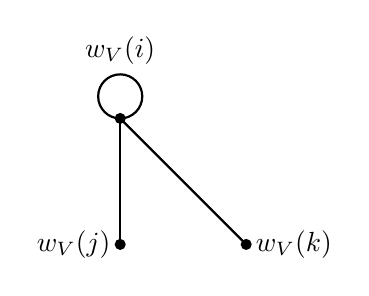
\begin{tikzpicture}
\begin{scope}[xscale=0.4, yscale=0.4]

\draw[thick](-2,2.7) circle [x radius=0.7cm, y radius=0.7cm];
\fill(-2,-2)circle (5pt);
\fill(-2,2)circle (5pt);
\fill(2,-2)circle (5pt);
\draw[thick](-2,-2)--(-2,2);
\node[above] at (-2,3.4) {$w_{V}(i)$};
\draw[thick](2,-2)--(-2,2);
\node[left] at (-2,-2) {$w_{V}(j)$};
\node[right] at (2,-2) {$w_{V}(k)$};

\end{scope}
\end{tikzpicture}
\caption{}
\label{three_vertices2} 
\end{figure}
However, we have that 
\begin{align*}
\{w_{V}(i), w_{E}(ij), w_{E}(ik)\}=
\{w_{V}(i), w_{V}(i)-w_{V}(j), w_{V}(i)-w_{V}(k)\} 
\end{align*}
is linearly independent. 
Therefore, this is not $2$-independent.
Similarly, it is easy to verify that the other cases are not $2$-independent. 
We can also check that the graph consisting of three loops is not  $2$-independent.
Therefore, we complete the case when $\Gamma'$ has three vertices.

If $\Gamma'$ consists of two vertices, then by the definition of weighted signed graph  there are the following possibilities for $i<j$ as in Figure~\ref{two_vertices}.
%%%%%%%%%%%%%%%%%%%%%%%%%%%%%%%%%%%%%%%%%%%%%%%%%%%%%%%%%%%%%%%%%%%%%%%%%%%
% Figure 7
%%%%%%%%%%%%%%%%%%%%%%%%%%%%%%%%%%%%%%%%%%%%%%%%%%%%%%%%%%%%%%%%%%%%%%%%%%%
\begin{figure}[h]
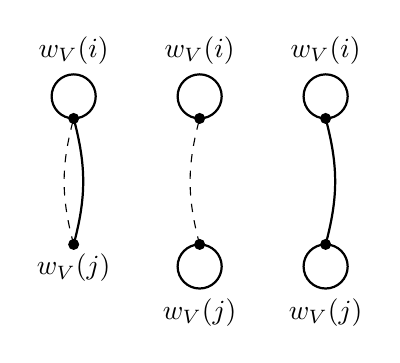
\begin{tikzpicture}
\begin{scope}[xscale=0.4, yscale=0.4]

\fill(2,2)circle (5pt);
\fill(2,-2)circle (5pt);
\draw[thick](2,-2)to[out=75,in=-75](2,2);
\draw[dashed](2,-2)to[out=105,in=-105](2,2);
\draw[thick](2,2.7) circle [x radius=0.7cm, y radius=0.7cm];
\node[above] at (2,3.4) {$w_{V}(i)$};
\node[below] at (2,-2) {$w_{V}(j)$};

\fill(6,2)circle (5pt);
\fill(6,-2)circle (5pt);
\draw[dashed](6,-2)to[out=105,in=-105](6,2);
\draw[thick](6,2.7) circle [x radius=0.7cm, y radius=0.7cm];
\node[above] at (6,3.4) {$w_{V}(i)$};
\draw[thick](6,-2.7) circle [x radius=0.7cm, y radius=0.7cm];
\node[below] at (6,-3.4) {$w_{V}(j)$};

\fill(10,2)circle (5pt);
\fill(10,-2)circle (5pt);
\draw[thick](10,-2)to[out=75,in=-75](10,2);
\draw[thick](10,2.7) circle [x radius=0.7cm, y radius=0.7cm];
\node[above] at (10,3.4) {$w_{V}(i)$};
\draw[thick](10,-2.7) circle [x radius=0.7cm, y radius=0.7cm];
\node[below] at (10,-3.4) {$w_{V}(j)$};

\end{scope}
\end{tikzpicture}
\caption{} 
\label{two_vertices}
\end{figure}

From the left, the weights on the loops and edges consist of the following set:
\begin{align*}
& \{e_{i}, e_{i}+e_{j}, e_{i}-e_{j}\}\ {\rm or}\ \{2e_{i}, e_{i}+e_{j}, e_{i}-e_{j}\}; \\
& \{e_{i}, e_{i}+e_{j}, e_{j}\}\ {\rm or}\ \{2e_{i}, e_{i}+e_{j}, 2e_{j}\}; \\
& \{e_{i}, e_{i}-e_{j}, e_{j}\}\ {\rm or}\ \{2e_{i}, e_{i}-e_{j}, 2e_{j}\}.
\end{align*}
All of them are $2$-independent.
Consequently, if $\Gamma'$ consists of two vertices, then it must be the last three graphs in Figure~\ref{example_weighted_vertex}.
\end{proof}

\end{document}
